\documentclass{skripsi}

\newcommand{\JudulSkripsi}{PROTOTIPE SISTEM DETEKSI DAN PENANGANAN
  CACAT PADA KONTAINER KIMIA UNTUK AREA INDUSTRI-TERISOLASI BERBASIS
ARTIFICIAL INTELLIGENCE DAN LENGAN ROBOT}
\newcommand{\NamaPenulis}{ALRIDHO}
\newcommand{\NIM}{H021211006}

\begin{document}
\newgeometry{top=22.5mm, bottom=22.5mm}
\definecolor{sampul}{HTML}{c80404}
\begin{titlepage}
  \begin{tikzpicture}[remember picture, overlay]
    \fill[sampul] (current page.south west) rectangle (current page.north east);
  \end{tikzpicture}

  \color{black}

  \vspace*{-0.7cm}

  \begin{center}
    \textbf{JUDUL BAHASA INDONESIA}
  \end{center}

  \vfill
  % Hexagon
  \begin{center}
    \begin{tikzpicture}[scale=1]
      \foreach \i/\x/\y in {
        1/3/3.2,
        2/7.8/3.2,
        3/0.6/4.6,
        4/5.4/4.6,
        5/3/6,
        6/5.4/7.4
      } {
        \begin{scope}[shift={(\x,\y)}]
          \clip (0:1.5) \foreach \a in {60,120,...,360} { -- (\a:1.5) };
          \node at (0,0) {\includegraphics[width=4cm]{gambar/img\i.jpg}};
          \draw[white, line width=1.5pt] (0:1.5) \foreach \a in
          {60,120,...,360} { -- (\a:1.5) } -- cycle;
        \end{scope}
      }
    \end{tikzpicture}
  \end{center}

  \vfill

  \begin{center}
    \textbf{ALRIDHO} \\
    \textbf{H021211006} \\[1cm]
  \end{center}

  \vfill

  \begin{minipage}{0.2\textwidth}
    \hspace*{-1cm}
    
\includegraphics[width=2.5cm]{gambar/uh-b.png}
  \end{minipage}
  \hfill
  \begin{minipage}{0.75\textwidth}
    \centering
    \textbf{PROGRAM STUDI FISIKA} \\
    \textbf{FAKULTAS MATEMATIKA DAN ILMU PENGETAHUAN ALAM} \\
    \textbf{UNIVERSITAS HASANUDDIN} \\
    \textbf{MAKASSAR} \\
    \textbf{2025}
  \end{minipage}

  \vspace*{0.5cm}

\end{titlepage}
\restoregeometry

\newgeometry{top=22.5mm, bottom=22.5mm}
\addcontentsline{toc}{chapter}{HALAMAN JUDUL}
\pagenumbering{roman}
\begingroup
\singlespacing
\fontsize{11pt}{13pt}\selectfont
\begin{center}
  \textbf{\JudulSkripsi} \\
  \vfill
  \textbf{\MakeTextUppercase{\NamaPenulis}} \\
  \textbf{\NIM} \\
  \vspace*{1.5cm}
  
\includegraphics[height=3.2cm]{gambar/uh-fc.png} \\
  \vfill
  \textbf{PROGRAM STUDI FISIKA} \\
  \textbf{FAKULTAS MATEMATIKA DAN ILMU PENGETAHUAN ALAM} \\
  \textbf{UNIVERSITAS HASANUDDIN} \\
  \textbf{MAKASSAR} \\
  \textbf{2025}
\end{center}
\endgroup
\restoregeometry

\newgeometry{top=22.5mm, bottom=22.5mm}
\addcontentsline{toc}{chapter}{HALAMAN PENGAJUAN}
\begingroup
\singlespacing
\fontsize{11pt}{13pt}\selectfont
\begin{center}
  \textbf{\JudulSkripsi} \\
  \vfill
  \NamaPenulis \\
  \NIM \\
  \vfill
  \begingroup
  \fontsize{10pt}{13pt}\selectfont
  Skripsi \\
  \vspace*{1cm}
  sebagai salah satu syarat untuk mencapai gelar sarjana \\
  \endgroup
  \vspace*{1cm}
  Program Studi Fisika \\
  \vfill
  pada \\
  \vfill
  \textbf{PROGRAM STUDI FISIKA} \\
  \textbf{FAKULTAS MATEMATIKA DAN ILMU PENGETAHUAN ALAM} \\
  \textbf{UNIVERSITAS HASANUDDIN} \\
  \textbf{MAKASSAR} \\
  \textbf{2025}
\end{center}
\endgroup
\restoregeometry

\backgroundsetup{
  scale=1,
  angle=0,
  opacity=0.2,
  position=current page.center,
  contents={
\includegraphics[width=7cm,height=9cm]{gambar/uh-fc.png}}
}

\newgeometry{top=22.5mm, bottom=22.5mm}
\addcontentsline{toc}{chapter}{HALAMAN PENGESAHAN}
\begingroup
\singlespacing
\fontsize{11pt}{13pt}\selectfont
\begin{center}
  \textbf{SKRIPSI} \\
  \vfill
  \textbf{\JudulSkripsi} \\
  \vfill
  \textbf{\underline{\MakeTextUppercase{\NamaPenulis}}} \\
  \textbf{\NIM} \\
  \vfill
  \begingroup
  \fontsize{10pt}{13pt}\selectfont
  Skripsi, \\
  \vfill
  telah dipertahankan di depan Panitia Ujian Sarjana Xxxx pada
  tanggal bulan tahun dan dinyatakan telah memenuhi syarat kelulusan \\
  pada \\
  \vfill
  Program Studi Fisika \\
  Departemen Fisika \\
  Fakultas Matematika dan Ilmu Pengetahuan Alam \\
  Universitas Hasanuddin \\
  Makassar \\
  \vfill
  \noindent
  \begin{minipage}[t]{0.38\textwidth}
    Mengesahkan:\par
    Pembimbing tugas akhir,\par\vspace{2cm}

    \underline{\NamaPembimbing}\\
    NIP. 19670520 199403 1 002
  \end{minipage}
  \hfill
  \begin{minipage}[t]{0.38\textwidth}
    Mengetahui:\par
    Ketua Program Studi,\par\vspace{2cm}

    \underline{Prof. Dr. Arifin, M.T}\\
    NIP. 19670520 199403 1 002
  \end{minipage}
  \endgroup
\end{center}

\endgroup
\restoregeometry
\clearpage
\backgroundsetup{contents={}}

\begingroup
\singlespacing
\chapter*{PERNYATAAN KEASLIAN SKRIPSI}
\addcontentsline{toc}{chapter}{LEMBAR PERNYATAAN KEASLIAN SKRIPSI}
\noindent
Dengan ini saya menyatakan bahwa, skripsi berjudul “\textbf{\JudulSkripsi}”
adalah benar karya saya dengan arahan dari pembimbing (Prof. Dr.
Arifin, M.T). Karya ilmiah ini belum diajukan dan tidak sedang
diajukan dalam bentuk apapun kepada perguruan tinggi mana pun. Sumber
inf ormasi yang berasal atau dikutip dari karya yang diterbitkan
maupun tidak diterbitkan dari penulis lain telah disebutkan dalam
teks dan dicantumkan dalam Daf tar Pustaka skripsi ini. Apabila di
kemudian hari terbukti atau dapat dibuktikan bahwa sebagian atau
keselurusan skripsi ini adalah karya orang lain, maka saya bersedia
menerima sanksi atas perbuatan tersebut berdasarkan aturan yang berlaku. \par

\noindent
\\
Dengan ini saya melimpahkan hak cipta (hak ekonomis) dari karya tulis
saya berupa skripsi ini kepada Universitas Hasanuddin. \par

\vspace{2cm}

\hfill
\begin{minipage}{0.4\textwidth}
  \raggedleft
  Makassar, XX Juni 2025 \par
  \vspace{2cm}
  Alridho \\
  H021211006
\end{minipage}
\endgroup

\begingroup
\chapter*{UCAPAN TERIMA KASIH}
\addcontentsline{toc}{chapter}{UCAPAN TERIMA KASIH}
% \lipsum[1] \par
% \lipsum[2] \par
% Lorem ipsum dolor sit amet, consectetur adipiscing elit. Fusce
% malesuada non dui quis condimentum. Etiam dapibus ligula sapien:
% \begin{enumerate}
%   \item Items are numbered automatically.
%   \item The numbers start at 1 with each use of the
%     \texttt{enumerate} environment.
%   \item Another entry in the list.\\
% \end{enumerate}

\noindent
Segala puji dan syukur penulis panjatkan kehadirat Allah Subhanahu Wa
Ta’ala atas segala berkah, rahmat, dan karunia-Nya yang telah
memberikan ilmu pengetahuan, pengalaman, kekuatan, kesabaran, dan
kesempatan kepada penulis sehingga mampu menyelesaikan skripsi ini.
Penulisan skripsi yang berjudul \textbf{"\JudulSkripsi"} merupakan
upaya penulis memenuhi salah satu syarat dalam menyelesaikan pendidikan dan
memperoleh gelar Sarjana Sains di Departemen Fisika, Fakultas
Matematika dan Ilmu Pengetahuan Alam, Universitas Hasanuddin. Selain
itu, skripsi ini juga diharapkan dapat memberikan manfaat bagi
pembaca dan peneliti lain untuk menambah wawasan dalam bidang fisika
khususnya elektronika dan instrumentasi.

Proses penyelesaian skripsi ini merupakan suatu rangkaian perjuangan
yang cukup panjang bagi penulis. Selama proses penelitian maupun
penyusunan skripsi ini, tidak sedikit hambatan maupun kendala yang
penulis hadapi. Do’a dan dukungan dari berbagai pihak merupakan hal
yang berarti, sehingga penyusunan skripsi ini dapat diselesaikan oleh
penulis. Oleh karena itu, dengan tulus dan ikhlas, penulis
mengucapkan terima kasih sebanyak-banyaknya.

Penulis menyampaikan penghargaan setinggi-tingginya dan banyak terima
kasih kepada Bapak \textbf{Prof. Dr. Arifin, M.T} selaku pembimbing saya atas
kesediannya telah meluangkan banyak waktu, tenaga dan pikiran dalam
memberikan bimbingan dan motivasi kepada Penulis, mulai dari awal
penyusunan sampai penyelesaian skripsi ini. Pada kesempatan ini pula,
dengan segala kerendahan hati Penulis ingin menyampaikan ucapan
terima kasih yang sebesar-besarnya kepada:

\begin{enumerate}
  \item Keluarga tercinta, khususnya kedua orang tua saya, Ayahanda
    \textbf{Muh. Anto} dan Ibunda \textbf{Nuraeni}, yang telah
    memberikan dukungan materiil dan moril serta tak henti mendoakan.
    Terima kasih juga untuk adik saya, Cinta Kasih Rahmadany, yang
    turut memberi semangat dalam menyelesaikan perjalanan ini.
  \item Dosen penguji kak \textbf{Ida Laila, S.Si., M.Si.} dan Ibu
    \textbf{Prof. Dr. Sri Suryani, DEA.} atas kesediaannya untuk
    meluangkan waktu, menguji, serta memberikan kritik dan saran yang
    sangat berharga untuk skripsi ini.
  \item Bapak dan Ibu \textbf{Dosen Pengajar Departemen Fisika Fakultas
    Matematika dan Ilmu Pengetahuan Alam Universitas Hasanuddin},
    terima kasih atas ilmu dan bimbingannya selama ini. Semoga hasil
    ajaran Bapak dan Ibu selalu memberikan manfaat bagi setiap orang.
  \item Bapak dan Ibu Staf Departemen Fisika khususnya \textbf{Pak Syukur},
    Ibu \textbf{Evi}, dan Kak \textbf{Rana} yang selalu membantu penulis
    selama berada di kampus.
  \item Teman-teman seperjuangan di kampus \textbf{Ragil, Vivaldo, Salim,
    Werdi, Adri, Akmal, dan lain-lain} atas kebersamaannya di dalam
    dan di luar kampus.
  \item Seluruh pihak yang telah membantu dan memberikan dukungan
    yang tidak dapat penulis sebutkan namanya satu per satu.
\end{enumerate}

Penulis berharap semoga segala kebaikan yang diberikan dari berbagai
pihak kepada penulis untuk menyelesaikan skripsi ini dapat bernilai
ibadah. Akhir kata, penulis memohon maaf atas kesalahan yang
disengaja maupun tidak disengaja dalam rangkaian penyusunan skripsi
ini. Semoga skripsi ini dapat memberikan manfaat bagi pembaca.

\vspace{2cm}

\hfill
\begin{minipage}{0.4\textwidth}
  \raggedleft
  Makassar, \today \par
  \vspace{2cm}
  Alridho \\
  H021211006
\end{minipage}
\endgroup

\begingroup
\singlespacing
\chapter*{ABSTRAK}
\addcontentsline{toc}{chapter}{ABSTRAK}

\noindent
Alridho. \textbf{JUDUL BAHASA INDONESIA} (dibimbing oleh Prof. Dr. Arifin, M.T.). \par

\vspace*{0.1cm}

\noindent
\textbf{Latar Belakang}. Inspeksi manual pada kontainer kimia di industri memiliki tingkat kesalahan yang tinggi, berkisar antara 20\% hingga 30\%, dan menimbulkan risiko paparan zat berbahaya bagi pekerja. \textit{Artificial Intelligence} (AI) dan robotika dapat meningkatkan efisiensi, keamanan, dan produktivitas. Model deteksi cacat seperti \textit{autoencoder} sangat efektif karena mampu belajar dari data normal untuk mengidentifikasi anomali, yang sangat berguna ketika data cacat sulit diperoleh. \textbf{Tujuan}. Penelitian ini bertujuan untuk (1) merancang model deteksi objek berbasis YOLO untuk mengenali kontainer kimia secara akurat, (2) membangun model deteksi kecacatan menggunakan algoritma convolutional autoencoder (CVAE) yang efektif, dan (3) mengintegrasikan kedua model tersebut ke dalam sistem lengan robot untuk identifikasi dan penyortiran otomatis. \textbf{Metode}. Penelitian ini menggunakan pendekatan eksperimental dengan merancang prototipe yang terdiri dari perangkat keras dan lunak. Perangkat keras utama meliputi lengan robot, Arduino Uno, motor servo, sensor PIR, dan kamera. Prosesnya dimulai saat kamera menangkap citra kontainer. Model YOLO kemudian mendeteksi objek kontainer dari citra tersebut. Selanjutnya, model CVAE menganalisis citra untuk menentukan ada atau tidaknya cacat dengan menghitung \textit{reconstruction error}. Berdasarkan hasil analisis, lengan robot secara otomatis menyortir kontainer ke area "cacat" atau "normal". Ambang batas untuk penentuan cacat ditetapkan sebesar 0,007183 melalui analisis kurva ROC. \textbf{Hasil}. Hasil penelitian menunjukkan model deteksi objek YOLO berhasil dilatih dengan performa sangat tinggi, di mana nilai mAP@50 mendekati 1.00. Model deteksi kecacatan CVAE, setelah dilatih, mampu membedakan kontainer cacat dan normal secara efektif. Pengujian sistem secara menyeluruh sebanyak 25 kali pada sampel uji menunjukkan bahwa prototipe mampu mengklasifikasikan dan menyortir kontainer dengan tingkat akurasi 100\%. Seluruh proses, termasuk jumlah kontainer yang diinspeksi dan tingkat kecacatan, berhasil ditampilkan secara \textit{real-time} melalui berbasis \textit{web}. \textbf{Kesimpulan}. Prototipe sistem inspeksi visual cerdas ini berhasil mendemonstrasikan kelayakannya untuk otomasi penuh di lingkungan industri terisolasi. Sistem ini berhasil menggabungkan model deteksi objek YOLO yang akurat, model deteksi kecacatan CVAE yang efektif dengan akurasi 100\% pada data uji, serta sistem penyortiran fisik menggunakan lengan robot secara terintegrasi dan otomatis. \par 

\vspace*{0.1cm}

\noindent
\textbf{Kata Kunci:} Deteksi cacat; prototipe; lengan robot; YOLO; autoencoder; IoT.

\endgroup

\newpage

\begingroup
\singlespacing
\chapter*{ABSTRACT}
\addcontentsline{toc}{chapter}{ABSTRACT}

\noindent
Alridho. \textbf{JUDUL BAHASA INGRRIS} (dibimbing oleh Prof. Dr. Arifin, M.T.). \par

\vspace*{0.1cm}
 
\noindent
\lipsum[1]


\vspace*{0.1cm}

\noindent
\textbf{Kata Kunci:} Prototipe; monitoring; IoT; sensor; telegram.

\endgroup


\newpage
\chapter*{DAFTAR ISI}
\noindent\hfill\textbf{Halaman}
\addcontentsline{toc}{chapter}{DAFTAR ISI}
\tableofcontents

\chapter{Pendahuluan}
\section{Latar Belakang}
    Lorem ipsum dolor sit amet, consectetur adipiscing elit. Fusce malesuada non dui quis condimentum. Etiam dapibus ligula sapien, sed malesuada nisi lacinia finibus. Maecenas pulvinar mauris quis lorem vehicula porttitor. Vestibulum in eleifend tortor. Morbi hendrerit diam dui, mattis egestas elit mollis eu. Phasellus a venenatis elit, a euismod lacus. Nullam nec placerat magna. Quisque ligula tortor, rhoncus vitae finibus sit amet, laoreet commodo quam. In placerat semper tellus, nec ultrices diam sodales non. Quisque ut varius ligula. Aenean accumsan felis et metus blandit lobortis. Maecenas ut eros vel eros scelerisque scelerisque dictum quis leo. Donec lacinia erat in arcu tincidunt luctus. Duis bibendum, justo a interdum maximus, velit sem tincidunt diam, quis dignissim felis leo ut nunc.\par

    Suspendisse sed est ut risus finibus faucibus. Integer nisl ex, efficitur vel commodo sit amet, mollis vel dolor. Phasellus quis mauris vestibulum, hendrerit felis non, sollicitudin dolor. Etiam sodales aliquam nibh vitae auctor. Nunc gravida varius mauris, bibendum placerat odio lacinia vitae. Aenean non porttitor augue. Lorem ipsum dolor sit amet, consectetur adipiscing elit. Suspendisse vel ante laoreet, consequat justo finibus, eleifend urna. Suspendisse potenti. Curabitur felis libero, suscipit eget pulvinar pharetra, tristique ac ipsum. \par

    Suspendisse potenti. Phasellus nec semper nulla. Cras sed ligula vel mi faucibus maximus in sed erat. Vestibulum ante ipsum primis in faucibus orci luctus et ultrices posuere cubilia curae; Ut eget dignissim massa. Phasellus orci orci, vehicula at consectetur id, tincidunt vitae nibh. Interdum et malesuada fames ac ante ipsum primis in faucibus. Nullam elit orci, volutpat eleifend quam sed, aliquam tristique odio. Phasellus orci mi, aliquam non odio nec, volutpat molestie elit. Maecenas ex massa, efficitur in tincidunt sit amet, venenatis et mauris. Praesent sollicitudin tempor arcu, semper condimentum massa molestie sit amet.\par

    Mauris ornare leo aliquet pulvinar euismod. Donec consectetur luctus orci, eget cursus neque aliquet ac. Vestibulum quis vestibulum felis. Cras vitae erat et lorem blandit dictum. Phasellus feugiat fermentum purus non lacinia. Sed eleifend dui id massa placerat porttitor. Vivamus commodo, dui eu ornare blandit, elit ante imperdiet mi, in euismod dolor dolor ut sapien. Suspendisse potenti. Fusce pellentesque, lacus vel consequat mattis, nisi augue efficitur ligula, a porttitor arcu magna id dui. Vivamus sed leo molestie, viverra nulla nec, tempor mi. Pellentesque tincidunt ipsum a luctus viverra. Orci varius natoque penatibus et magnis dis parturient montes, nascetur ridiculus mus.\par

    Aliquam vel lectus ipsum. Duis nec nulla magna. Nunc nec mauris ornare, vestibulum nulla vel, finibus nibh. Mauris et nisi pellentesque, eleifend lectus et, tempor nulla. Duis in quam ultricies lacus vehicula dictum. Vestibulum pretium neque eu porta elementum. Maecenas non velit consequat, eleifend turpis vitae, efficitur tellus. Duis velit felis, vulputate vitae ipsum non, lobortis condimentum nibh. Etiam vitae aliquet sem. Vivamus feugiat arcu lectus, bibendum rutrum justo placerat a. \par

\chapter{METODE PENELITIAN}
\section{Tempat dan Waktu Penelitian}
Penelitian ini dilaksanakan mulai dari bulan Februari 2025 hingga Juni
2025, bertempat di Laboratorium Elektronika dan Instrumentasi,
Departemen Fisika, Fakultas Matematika dan Ilmu Pengetahuan Alam,
Universitas Hasanuddin, Makassar.

\vspace{1em}

\section{Peralatan Penelitian}
Adapun peralatan yang digunakan pada penelitian ini adalah sebagai berikut:
\begin{enumerate}
  \item Arduino Uno berfungsi sebagai mikrokontroler utama yang
    mengendalikan motor \textit{servo} pada lengan robot serta menerima sinyal
    dari sensor.
  \item Motor \textit{servo} digunakan sebagai aktuator untuk menggerakkan
    bagian-bagian lengan robot sesuai perintah dari Arduino.
  \item Lengan robot EEZYbotARM MK1 berfungsi sebagai struktur
    mekanik yang menjadi tempat pemasangan motor \textit{servo} dan berperan
    sebagai sistem pergerakan robotik.
  \item \textit{Power supply} 5V berfungsi memberikan catu daya stabil untuk
    motor \textit{servo} agar dapat beroperasi dengan baik.
  \item \textit{Sensor Passive Infrared Receiver} (PIR) HC-SR501
    digunakan untuk mendeteksi gerakan dan membantu
    menghitung jumlah kontainer cacat dan non-cacat yang lewat.
  \item Kamera digunakan untuk mengambil gambar kontainer kimia, yang
    kemudian diproses oleh model deteksi (YOLO) dan deteksi cacat
    (\textit{autoencoder}).
  \item Laptop/komputer digunakan untuk mengunggah program ke Arduino
    Uno, serta menjalankan model deteksi berbasis YOLO dan
    \textit{autoencoder} untuk analisis visual.
  \item Kabel \textit{jumper} berfungsi menghubungkan berbagai komponen
    elektronik seperti sensor dan aktuator ke papan rangkaian dan
    Arduino.
  \item Papan rangkaian berfungsi untuk menyediakan jalur koneksi
    antar komponen.
\end{enumerate}

\vspace{1em}

\section{Metode Kerja}
Dalam penelitian ini terdapat beberapa tahapan yang harus dilakukan.
Tahapan penelitian secara lengkap dapat dilihat pada
\textit{flowchart} yang tertera pada
Gambar \ref{fig:bagan-umum}. Penelitian ini dibatasi pada perancangan
dan pembuatan prototipe sistem deteksi cacat otomatis.

% \begin{figure}[H]
%   \centering
%   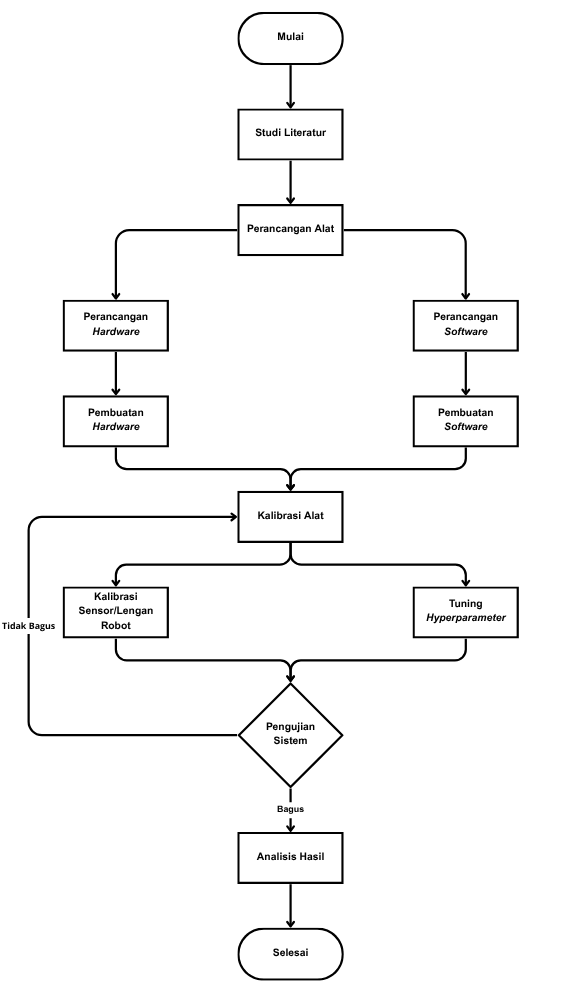
\includegraphics[width=0.7\textwidth]{gambar/bagan-umum.png}
%   \caption{Bagan alir penelitian}
%   \label{fig:bagan-umum}
% \end{figure}
% \vspace{-1em}

\begin{figure}[H]
  \centering
  \begin{tikzpicture}[
      every node/.style={font=\fontsize{9}{11}\selectfont},
      node distance = 0.77cm and 1cm
    ]
    \node (mulai) [startstop] {Mulai};
    \node (literatur) [process, below=of mulai] {Studi Literatur};
    \node (perancangan-alat) [process, below=of literatur] {Perancangan Alat};
    \node (perancangan-hardware) [process, align=center, below
    left=of perancangan-alat]
    {Perancangan \\ \textit{Hardware}};
    \node (perancangan-software) [process, align=center, below
    right=of perancangan-alat]
    {Perancangan \\ \textit{Software}};
    \node (pembuatan-hardware) [process, align=center, below=of
    perancangan-hardware]
    {Pembuatan \\ \textit{Hardware}};
    \node (pembuatan-software) [process, align=center, below=of
    perancangan-software]
    {Pembuatan \\ \textit{Software}};
    \coordinate (merge1) at
    ($(pembuatan-hardware.south)!0.5!(pembuatan-software.south)$);
    \node (kalibrasi-alat) [process, align=center, below=of merge1,
    yshift=-0.5cm] {Kalibrasi Alat};
    \node (kalibrasi-sensor) [process, align=center, below left=of
    kalibrasi-alat]
    {Kalibrasi \\ Sensor/Lengan Robot};
    \node (kalibrasi-parameter) [process, align=center, below
    right=of kalibrasi-alat]
    {\textit{Tuning} \\ \textit{Hyperparameter}};
    \coordinate (merge2) at
    ($(kalibrasi-sensor.south)!0.5!(kalibrasi-parameter.south)$);
    \node (pengujian-sistem) [decision, align=center, below=of
    merge2, yshift=-0.5cm] {Pengujian \\ Sistem};
    \node (analisis-hasil) [process, below=of pengujian-sistem]
    {Analisis Hasil};
    \node (selesai) [startstop, below=of analisis-hasil]
    {Selesai};

    % Arrow
    \draw [arrow] (mulai) -- (literatur);
    \draw [arrow] (literatur) -- (perancangan-alat);

    \draw [arrow] (perancangan-alat.west) -| (perancangan-hardware.north);
    \draw [arrow] (perancangan-alat.east) -| (perancangan-software.north);
    \draw [arrow] (perancangan-hardware) -- (pembuatan-hardware);
    \draw [arrow] (perancangan-software) -- (pembuatan-software);

    \draw [arrow] (pembuatan-hardware.south) --
    ($(pembuatan-hardware.south)+(0,-0.67cm)$) -| (kalibrasi-alat.north);
    \draw [arrow] (pembuatan-software.south) --
    ($(pembuatan-software.south)+(0,-0.67cm)$) -| (kalibrasi-alat.north);

    \draw [arrow] (kalibrasi-alat.south) --
    ($(kalibrasi-alat.south)+(0,-0.35cm)$) -| (kalibrasi-sensor.north);
    \draw [arrow] (kalibrasi-alat.south) --
    ($(kalibrasi-alat.south)+(0,-0.35cm)$) -| (kalibrasi-parameter.north);

    \draw [arrow] (kalibrasi-sensor.south) --
    ($(kalibrasi-sensor.south)+(0,-0.6cm)$) -| (pengujian-sistem.north);
    \draw [arrow] (kalibrasi-parameter.south) --
    ($(kalibrasi-parameter.south)+(0,-0.6cm)$) -| (pengujian-sistem.north);

    \draw [arrow] (pengujian-sistem.west) -- node[midway,
    yshift=0.25cm]{Tidak Bagus}
    ($(pengujian-sistem.west)+(-4.7cm,0)$) |- (kalibrasi-alat.west);
    \draw [arrow] (pengujian-sistem) -- node[midway, xshift=0.5cm]{Bagus}
    (analisis-hasil);

    \draw [arrow] (analisis-hasil) -- (selesai);

  \end{tikzpicture}
  \caption{Bagan alir penelitian}
  \label{fig:bagan-umum}
\end{figure}
\vspace{-1em}

Tahapan dimulai dengan kajian mendalam terhadap teknologi robotik,
algoritma \textit{autoencoder} untuk deteksi anomali visual, serta
metode deteksi objek seperti \textit{You Only Look Once} (YOLO), guna
memperoleh pemahaman komprehensif tentang konsep dasar, format
\textit{dataset}, dan teknik perancangan model untuk mendeteksi cacat
pada kontainer kimia. Setelah pemahaman awal diperoleh, dilakukan
perancangan sistem yang mencakup perangkat keras (lengan robot dan
sensor) serta perangkat lunak berupa algoritma \textit{machine
learning}. Selanjutnya, sistem robot dikalibrasi agar dapat bekerja
secara optimal, termasuk proses \textit{tuning hyperparameter} pada
model pembelajaran mesin. Jika sistem telah berfungsi sesuai dengan
yang diharapkan, maka dilanjutkan dengan proses pengambilan data
sebagai langkah awal dalam pengujian dan validasi model.

\vspace{1em}

\subsection{Perancangan \textit{Hardware}}
Penelitian ini dimulai dengan tahap perancangan \textit{hardware}. Komponen
\textit{hardware} yang digunakan meliputi kamera untuk mengambil gambar
kontainer kimia, laptop sebagai pusat pemrosesan dan eksekusi
algoritma pembelajaran mesin, serta sensor PIR untuk menghitung
jumlah kontainer kimia, baik yang cacat maupun yang tidak. Adapun
rancangan hardware dapat dilihat pada Gambar \ref{fig:rangkaian}.

\begin{figure}[H]
  \centering
  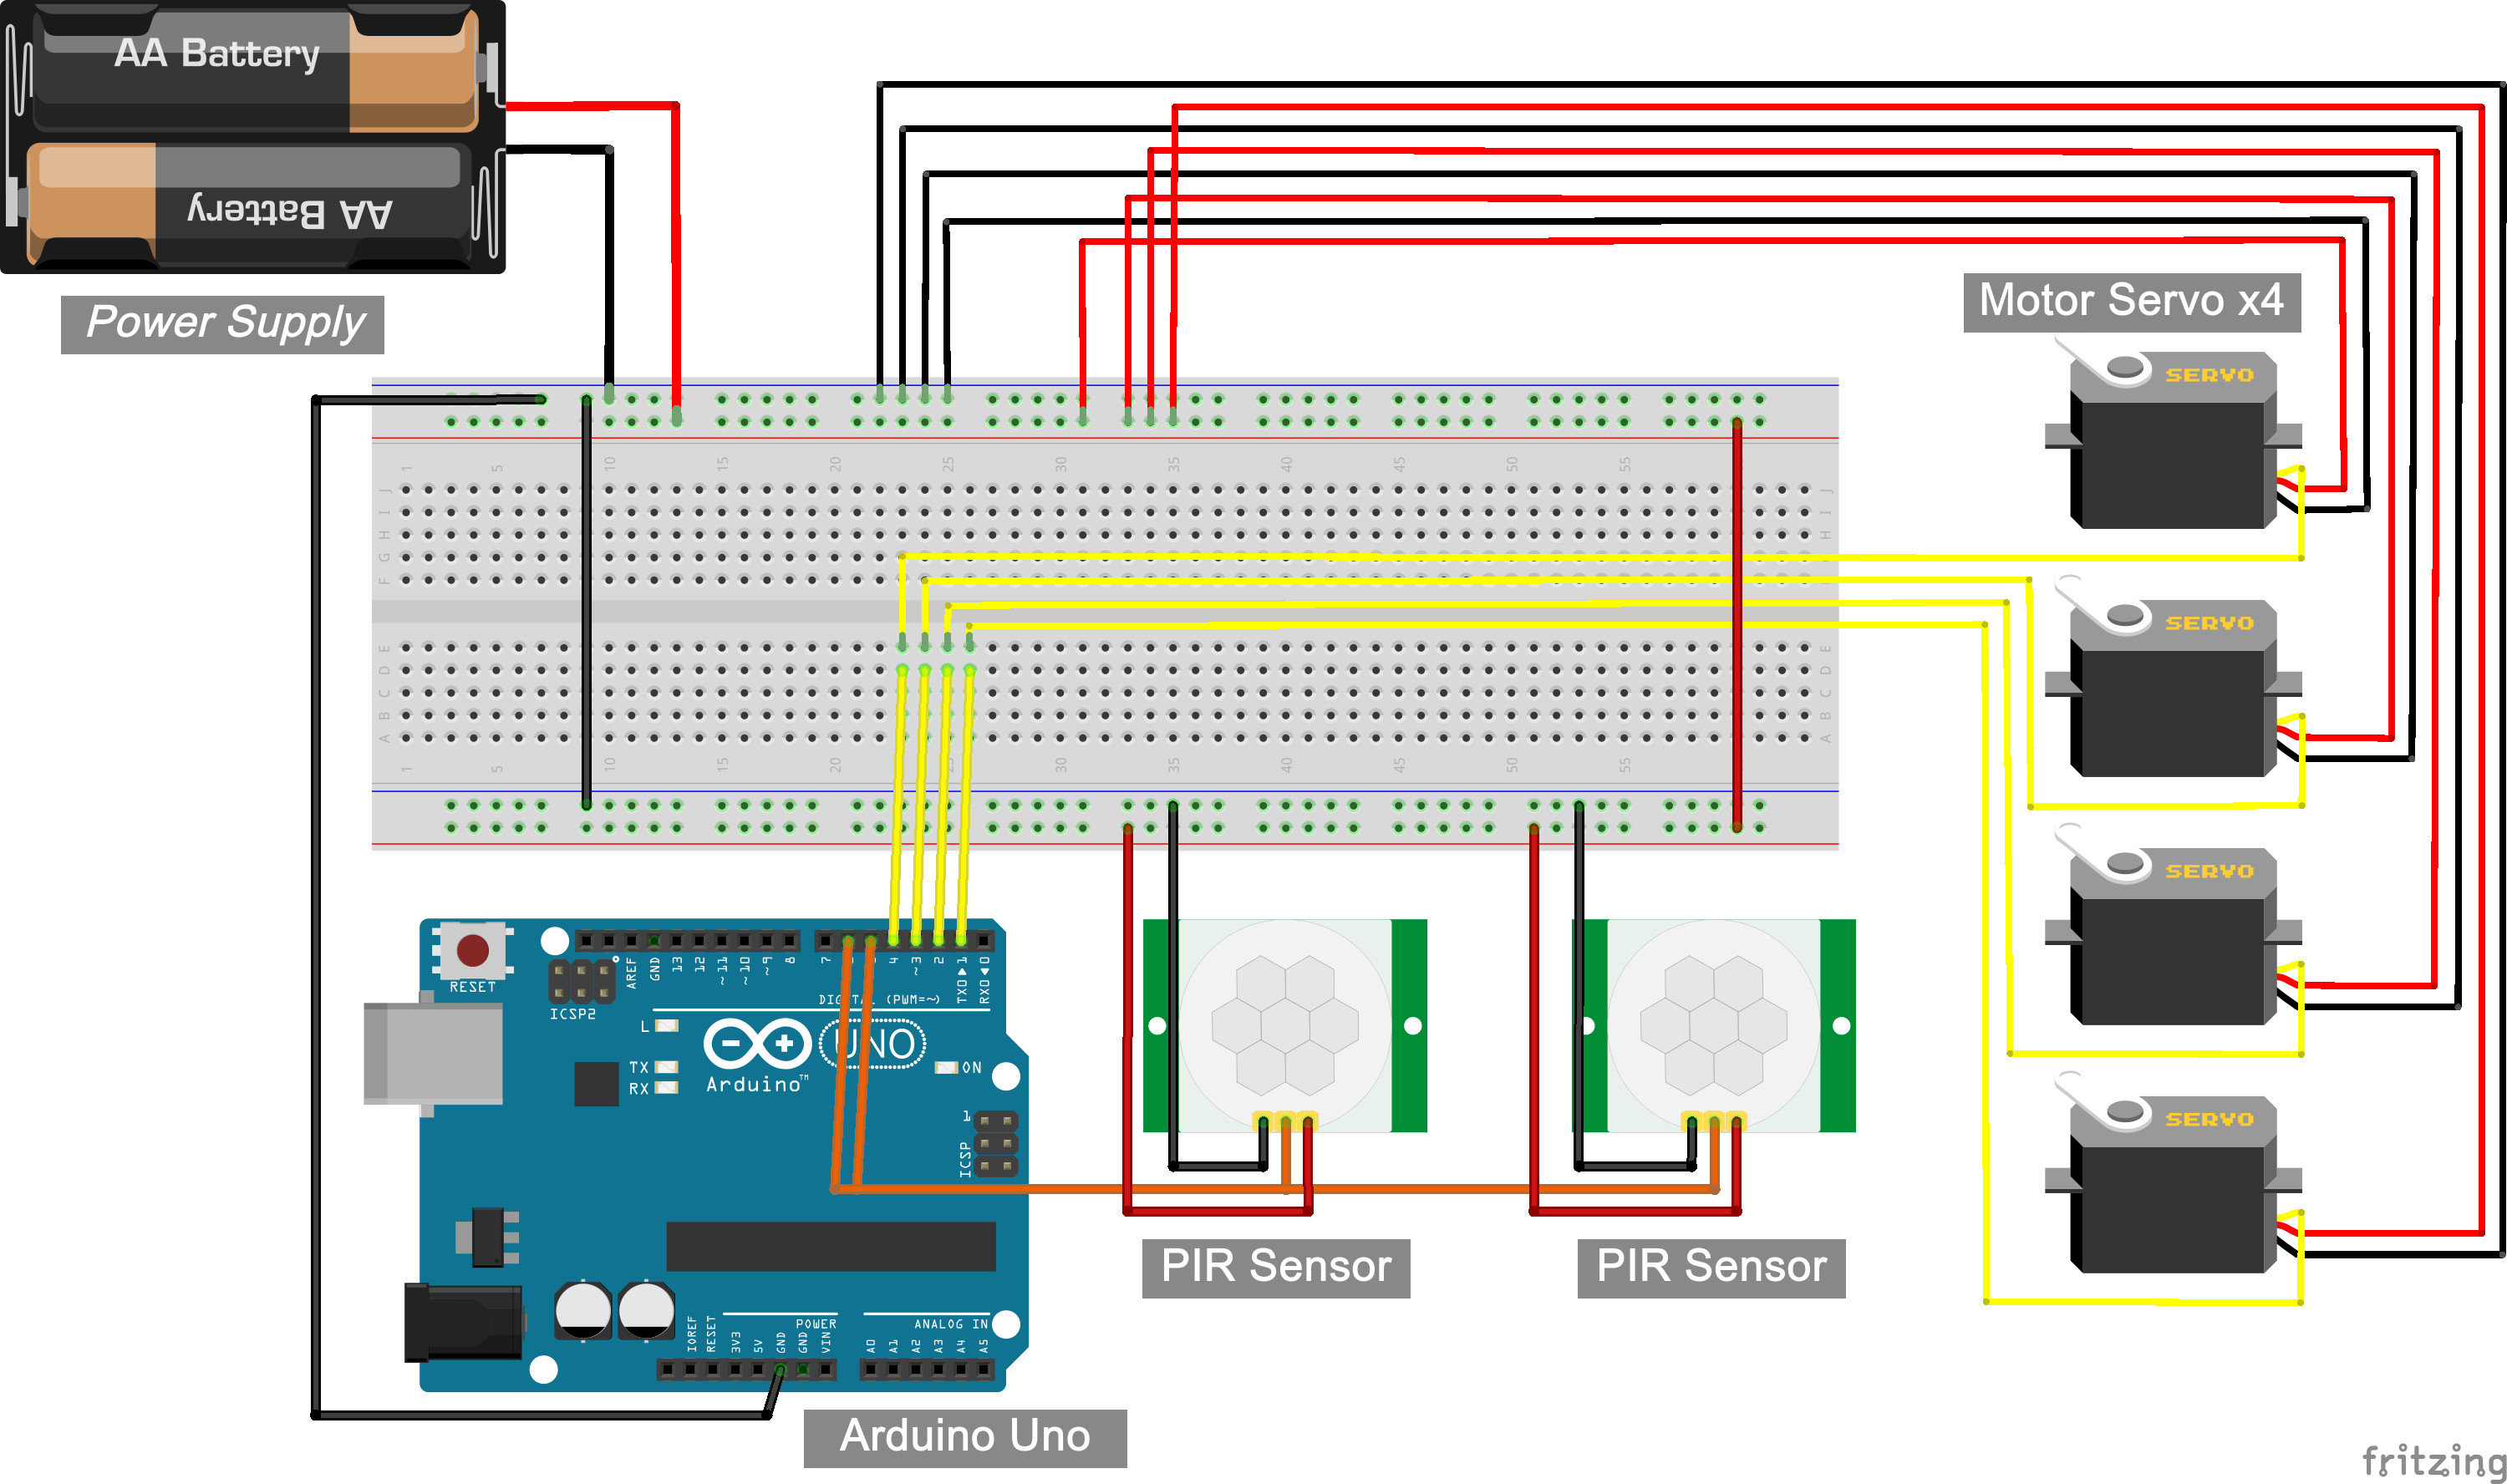
\includegraphics[width=\textwidth]{gambar/rangkaian.jpg}
  \caption{Rangkaian \textit{hardware} sistem}
  \label{fig:rangkaian}
\end{figure}
\vspace{-1em}

Sistem diawali saat kamera menangkap gambar kontainer kimia yang
diletakkan di area pengambilan gambar. Gambar ini diproses oleh model
deteksi objek (YOLO) untuk mengenali keberadaan kontainer sebelum
tahap deteksi cacat. Selanjutnya, gambar yang telah dikenali dikirim
ke model deteksi kecacatan berbasis \textit{convolutional variational
autoencoder} (CVAE) untuk
menentukan apakah kontainer mengalami cacat atau tidak. Berdasarkan
hasil analisis tersebut, sinyal dikirimkan ke mikrokontroler Arduino
untuk menggerakkan \textit{servo} sebagai respon terhadap kondisi kontainer.
Lengan robot kemudian mengambil kontainer kimia dan memindahkannya ke
wadah yang sesuai, tergantung pada hasil deteksi—apakah kontainer
tersebut cacat atau tidak. Untuk memantau dan menghitung jumlah
kontainer yang telah dipindahkan, dua sensor PIR dipasang pada
masing-masing wadah (cacat dan tidak). Data dari sensor ini
dikirim ke \textit{web server}, yang menyediakan API untuk dikonsumsi
agar data jumlah kontainer dapat ditampilkan ke klien secara
\textit{real-time}. Secara keseluruhan, keterkaitan antar komponen
perangkat keras dalam
sistem ini dapat dilihat pada Gambar \ref{fig:hardware}.

\begin{figure}[H]
  \centering
  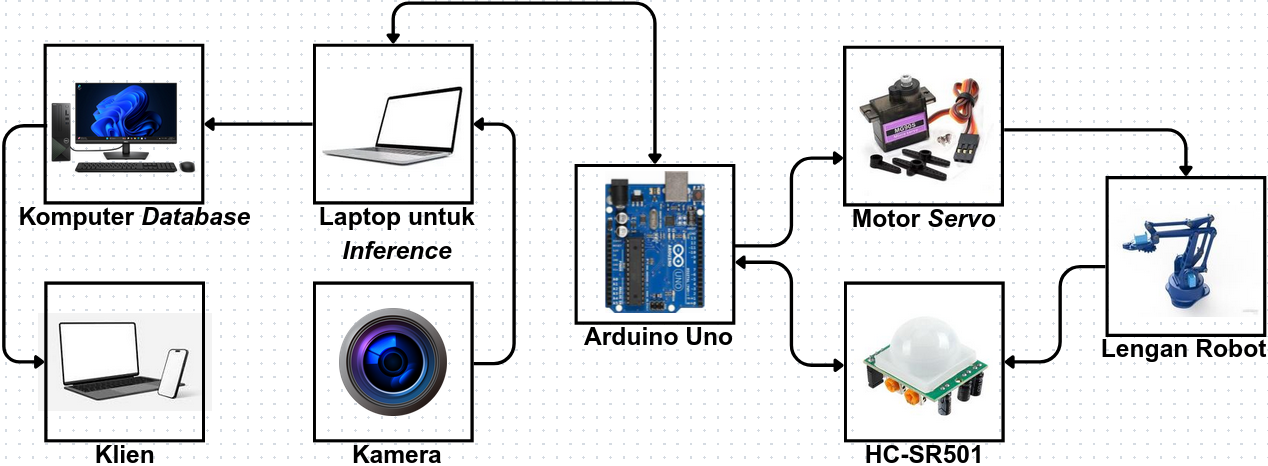
\includegraphics[width=\textwidth]{gambar/rancang.png}
  \caption{Rancang sistem \textit{hardware}}
  \label{fig:hardware}
\end{figure}
\vspace{-1em}

\vspace{1em}

\subsection{Perancangan \textit{Software}}
Perangkat lunak dalam penelitian ini mencakup perancangan beberapa
algoritma inti. Pertama, dirancang model deteksi objek berbasis YOLO
untuk mengenali kontainer kimia pada citra yang diambil oleh kamera.
Kedua, digunakan CVAE sebagai model untuk
mendeteksi cacat atau anomali visual pada kontainer. Selain itu,
dirancang pula algoritma kontrol untuk mengatur pergerakan lengan
robot dalam mengambil dan memindahkan kontainer berdasarkan hasil
klasifikasi. Sistem ini juga terintegrasi dengan modul
\textit{Internet of Things} (IoT) untuk menampilkan data kontainer
cacat dan non-cacat
pada klien secara \textit{real-time} melalui \textit{website}. \par

Tahap perancangan model deteksi objek dimulai dengan pengumpulan
\textit{dataset} berupa gambar kontainer kimia dari berbagai kondisi dan sudut
pandang menggunakan kamera, yang nantinya dipasang bersama lengan
robot. Setelah gambar terkumpul, dilakukan proses anotasi dengan
memberikan label dan \textit{bounding box} pada setiap kontainer sesuai dengan
format yang dibutuhkan oleh algoritma YOLO. \textit{Dataset} yang telah
dianotasi kemudian digunakan untuk melatih model deteksi objek.
Tujuannya agar model mampu mendeteksi kontainer kimia secara akurat
dan cepat dalam berbagai situasi, misalnya ketika kontainer berada
dalam posisi miring. Setelah proses pelatihan selesai, model
dievaluasi menggunakan data uji yang belum pernah dilihat sebelumnya.
Evaluasi dilakukan menggunakan beberapa metrik seperti \textit{precision},
\textit{recall}, dan \textit{mean Average Precision} (mAP), guna
memastikan bahwa model
memiliki kemampuan generalisasi yang baik dan layak diterapkan di
sistem robotik secara \textit{real-time}. \textit{Pipeline}
perancangan model deteksi
objek dapat dilihat pada Gambar \ref{fig:pipeline-yolo}.

% \begin{figure}[H]
%   \centering
%   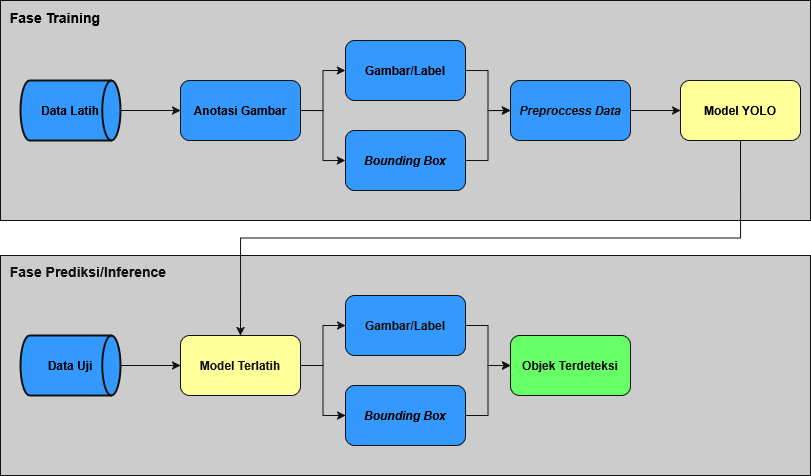
\includegraphics[width=\textwidth]{gambar/pipeline_yolo.png}
%   \caption{Diagram \textit{pipeline} pelatihan model YOLO}
%   \label{fig:pipeline-yolo}
% \end{figure}
% \vspace{-1em}

\begin{figure}[H]
  \centering
  \begin{tikzpicture}[
      every node/.style={font=\fontsize{8.5}{11}\selectfont},
      node distance = 0.5cm and 0.5cm
    ]
    % --- Pipeline pertama ---
    \node (data-latih1) [data] {Data Latih};
    \node (anotasi1) [pipeline-box, fill=cyan!50, right=of
    data-latih1] {Anotasi Gambar};
    \node (gambar-label1) [pipeline-box, fill=cyan!50, above right=of
    anotasi1] {Gambar/Label};
    \node (bounding-box1) [pipeline-box, fill=cyan!50, below right=of
    anotasi1] {\textit{Bounding Box}};
    \node (preprocess1) [pipeline-box, fill=cyan!50, above right=of
    bounding-box1] {\textit{Preprocess Data}};
    \node (yolo1) [pipeline-box, fill=yellow!50, right=of
    preprocess1] {Model Yolo};

    % Node dummy
    \node (start-bawah) [below=3cm of data-latih1] {};

    % --- Pipeline kedua ---
    \node (data-uji) [data, below=of start-bawah, xshift=1cm] {Data Uji};
    \node (model-terlatih) [pipeline-box, fill=yellow!50, right=of
    data-uji] {Model Terlatih};
    \node (gambar-label2) [pipeline-box, fill=cyan!50, above right=of
    model-terlatih] {Gambar/Label};
    \node (bounding-box2) [pipeline-box, fill=cyan!50, below right=of
    model-terlatih] {\textit{Bounding Box}};
    \node (objek-terdeteksi) [pipeline-box, fill=green!50, above
    right=of bounding-box2] {Objek Terdeteksi};

    % Arrow
    \draw [arrow] (data-latih1) -- (anotasi1);
    \draw [arrow] (anotasi1.east) -- ($(anotasi1.east)+(0.25cm, 0)$)
    |- (gambar-label1);
    \draw [arrow] (anotasi1.east) -- ($(anotasi1.east)+(0.25cm, 0)$)
    |- (bounding-box1);
    \draw [arrow] (gambar-label1.east) -- ($(gambar-label1.east)+(0.20cm, 0)$)
    |- (preprocess1);
    \draw [arrow] (bounding-box1.east) -- ($(bounding-box1.east)+(0.20cm, 0)$)
    |- (preprocess1);
    \draw [arrow] (preprocess1) -- (yolo1);

    \draw [arrow] (data-uji) -- (model-terlatih);
    \draw [arrow] (model-terlatih.east) -- ($(model-terlatih.east)+(0.25cm, 0)$)
    |- (gambar-label2);
    \draw [arrow] (model-terlatih.east) -- ($(model-terlatih.east)+(0.25cm, 0)$)
    |- (bounding-box2);
    \draw [arrow] (gambar-label2.east) -- ($(gambar-label2.east)+(0.20cm, 0)$)
    |- (objek-terdeteksi);
    \draw [arrow] (bounding-box2.east) -- ($(bounding-box2.east)+(0.20cm, 0)$)
    |- (objek-terdeteksi);

    \draw [arrow] (yolo1.south) -- ($(yolo1.south)+(0,-1.9cm)$) -| (data-uji);
  \end{tikzpicture}
  \caption{Diagram \textit{pipeline} pelatihan model YOLO}
  \label{fig:pipeline-yolo}
\end{figure}
\vspace{-1em}

Berikutnya adalah tahap pembangunan model deteksi cacat menggunakan
algoritma CVAE. Tahap ini menggunakan
\textit{dataset}
yang sama seperti yang digunakan pada pelatihan model YOLO dengan
beberapa tambahan, namun
tanpa menggunakan anotasi \textit{bounding box} karena sifat
\textit{unsupervised} dari
\textit{autoencoder}. Data diproses melalui tahap \textit{preprocessing} seperti
\textit{resizing}, normalisasi, dan augmentasi (rotasi,
\textit{flipping}, pencahayaan)
untuk meningkatkan variasi. Model dirancang dengan dua komponen
utama: \textit{encoder} untuk mengekstraksi fitur penting dan menghasilkan
representasi berdimensi rendah (\textit{latent space}), serta
\textit{decoder} untuk
merekonstruksi gambar dari representasi tersebut. Setelah arsitektur
selesai dan data siap, model dilatih untuk meminimalkan perbedaan
antara gambar asli dan hasil rekonstruksi, sehingga mampu mengenali
citra normal secara akurat. Evaluasi dilakukan dengan menghitung
\textit{reconstruction error}, yang digunakan untuk membedakan antara gambar
normal dan cacat. Ambang batas deteksi ditentukan melalui analisis
distribusi \textit{error} pada data validasi. \textit{Pipeline}
perancangan model
deteksi cacat dapat dilihat pada Gambar \ref{fig:pipeline-autoencoder}.

% \begin{figure}[H]
%   \centering
%   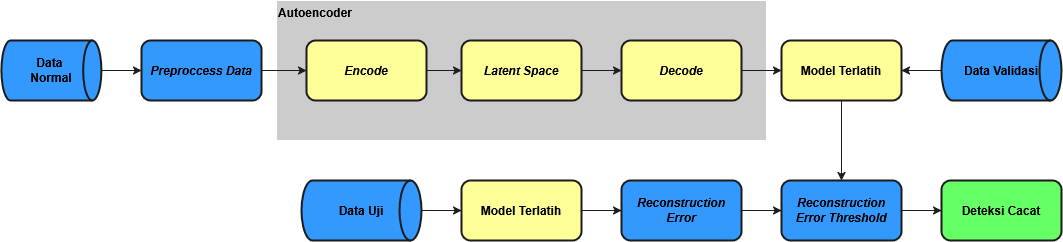
\includegraphics[width=\textwidth]{gambar/pipeline_autoencoder.png}
%   \caption{Diagram \textit{pipeline} pelatihan model deteksi cacat}
%   \label{fig:pipeline-autoencoder}
% \end{figure}
% \vspace{-1em}

\begin{figure}[H]
  \centering
  \begin{tikzpicture}[
      every node/.style={font=\fontsize{9}{11}\selectfont},
      node distance = 1cm and 2cm
    ]
    \node (data-normal) [data] {Data Normal};
    \node (preprocess) [pipeline-box, fill=cyan!50, below=of
    data-normal] {\textit{Preprocess Data}};
    \node (encode) [pipeline-box, fill=yellow!50, below=of
    preprocess] {\textit{Encode}};
    \node (latent-space) [pipeline-box, fill=yellow!50, below=of
    encode] {\textit{Latent Space}};
    \node (decode) [pipeline-box, fill=yellow!50, below=of
    latent-space] {\textit{Decode}};
    \node (model-terlatih) [pipeline-box, fill=yellow!50, below=of
    decode] {Model Terlatih};
    \node (data-validasi) [data, below=of
    model-terlatih] {Data Validasi};

    \node (data-uji) [data, left=of encode] {Data Uji};
    \node (model-terlatih2) [pipeline-box, fill=cyan!50, below=of
    data-uji] {Model Terlatih};
    \node (reconstruction) [pipeline-box, align=center, fill=cyan!50, below=of
    model-terlatih2]
    {\textit{Reconstruction} \\ \textit{Error}};
    \node (threshold) [pipeline-box, align=center, fill=cyan!50, below=of
    reconstruction]
    {\textit{Reconstruction Error} \\ \textit{Threshold}};
    \node (deteksi-cacat) [pipeline-box, fill=green!50, below=of
    threshold] {Deteksi Cacat};

    % Arrow
    \draw [arrow] (data-normal) -- (preprocess);
    \draw [arrow] (preprocess) -- (encode);
    \draw [arrow] (preprocess) -- (encode);
    \draw [arrow] (encode) -- (latent-space);
    \draw [arrow] (latent-space) -- (decode);
    \draw [arrow] (decode) -- (model-terlatih);
    \draw [arrow] (data-validasi) -- (model-terlatih);
    \draw [arrow] (data-uji) -- (model-terlatih2);
    \draw [arrow] (model-terlatih2) -- (reconstruction);
    \draw [arrow] (reconstruction) -- (threshold);
    \draw [arrow] (model-terlatih) -- (threshold);
    \draw [arrow] (threshold) -- (deteksi-cacat);
  \end{tikzpicture}
  \caption{Diagram \textit{pipeline} pelatihan model deteksi cacat}
  \label{fig:pipeline-autoencoder}
\end{figure}
\vspace{-1em}

\vspace{1em}

\subsection{Bagan Alir Sistem Kerja Alat}
Bagan alir kerja sistem secara keseluruhan dimulai saat kamera
menangkap citra, yang
kemudian diproses oleh model YOLO untuk mendeteksi objek kontainer.
Setelah terdeteksi, model \textit{autoencoder} menganalisis citra tersebut
untuk menentukan apakah terdapat kecacatan. Berdasarkan hasil
klasifikasi ini, lengan robot akan secara otomatis menyortir
kontainer ke lokasi yang telah ditentukan, yaitu ke area cacat jika
teridentifikasi cacat atau ke area normal jika sebaliknya.
Terakhir, informasi mengenai hasil penyortiran dikirimkan ke \textit{web
server} untuk keperluan pemantauan. Perancangan bagan alir sistem kerja
alat secara keseluruhan ditunjukkan pada Gambar \ref{fig:bagan-alir-kerja}.

% \begin{figure}[H]
%   \centering
%   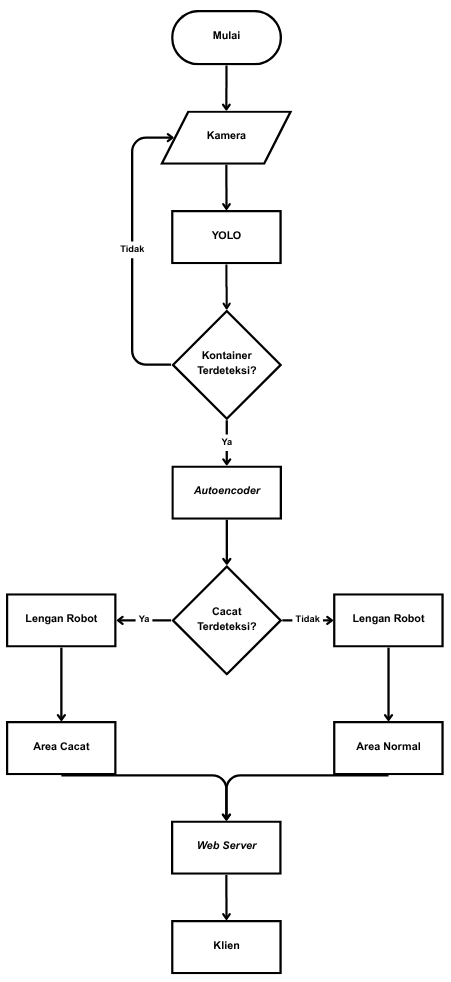
\includegraphics[width=0.7\textwidth]{gambar/flowchart.png}
%   \caption{Bagan alir sistem kerja alat}
%   \label{fig:bagan-alir-kerja}
% \end{figure}
% \vspace{-1em}

\begin{figure}[H]
  \centering

  \begin{tikzpicture}[
      every node/.style={font=\fontsize{9}{11}\selectfont},
      node distance = 0.75cm and 1.5cm
    ]
    \node (mulai) [startstop] {Mulai};
    \node (kamera) [input, below=of mulai] {Kamera};
    \node (yolo) [process, below=of kamera] {YOLO};
    \node (kontainer-terdeteksi) [decision, align=center, below=of yolo]
    {Kontainer \\ Terdeteksi?};
    \node (autoencoder) [process, below=of kontainer-terdeteksi]
    {\textit{Autoencoder}};

    \node (cacat-terdeteksi) [decision, align=center, below=of autoencoder]
    {Cacat \\ Terdeteksi?};
    \node (lengan-cacat) [process, left=of cacat-terdeteksi] {Lengan Robot};
    \node (area-cacat) [process, below=of lengan-cacat] {Area Cacat};
    \node (lengan-normal) [process, right=of cacat-terdeteksi] {Lengan Robot};
    \node (area-normal) [process, below=of lengan-normal] {Area Normal};

    \node (web) [process, below left=of area-normal] {\textit{Web Server}};
    \node (klien) [process, below=of web] {Klien};
    \node (selesai) [startstop, below=of klien] {Selesai};

    % Arrow
    \draw [arrow] (mulai) -- (kamera);
    \draw [arrow] (kamera) -- (yolo);
    \draw [arrow] (yolo) -- (kontainer-terdeteksi);

    \draw [arrow] (kontainer-terdeteksi) -- node[midway,
    xshift=0.3cm]{Iya} (autoencoder);
    \draw [arrow] (kontainer-terdeteksi.west) -- node[midway,
    yshift=0.25cm]{Tidak}
    ($(kontainer-terdeteksi.west)+(-2cm,0)$) |- (kamera.west);

    \draw [arrow] (autoencoder) -- (cacat-terdeteksi);
    \draw [arrow] (cacat-terdeteksi.east) -- node[midway, yshift=0.25cm]{Tidak}
    (lengan-normal);
    \draw [arrow] (cacat-terdeteksi.west) -- node[midway,
    yshift=0.25cm]{Iya} (lengan-cacat);
    \draw [arrow] (lengan-cacat) -- (area-cacat);
    \draw [arrow] (lengan-normal) -- (area-normal);

    \draw [arrow] (area-cacat.south) --
    ($(area-cacat.south)+(0,-0.4)$) -| (web.north);
    \draw [arrow] (area-normal.south) --
    ($(area-normal.south)+(0,-0.4)$) -| (web.north);

    \draw [arrow] (web) -- (klien);
    \draw [arrow] (klien) -- (selesai);

  \end{tikzpicture}
  \caption{Bagan alir sistem kerja alat}
  \label{fig:bagan-alir-kerja}
\end{figure}
\vspace{-1em}

\chapter{HASIL DAN PEMBAHASAN}
\section{Hasil Perancangan Sistem}
Sistem deteksi kecacatan kontainer ini dirancang secara otomatis
menggunakan kamera sebagai sensor utama dan lengan robot sebagai
aktuator. Proses diawali dengan model YOLO yang mengidentifikasi
keberadaan kontainer dari input kamera. Jika kontainer terdeteksi,
citra akan dianalisis oleh model Autoencoder untuk mengklasifikasikan
adanya kecacatan. Berdasarkan hasil klasifikasi tersebut, lengan
robot yang digerakkan servo akan menyortir kontainer ke dalam
kategori cacat atau non-cacat. Secara terpisah, sensor PIR
(\textit{Passive Infrared}) berfungsi menghitung jumlah total
kontainer pada setiap kategori, di mana data tersebut kemudian
dikirim (POST) ke server untuk visualisasi pada sisi klien. Desain
sistem yang dirancang diilustrasikan pada Gambar x.

\vspace{1em}

\section{Hasil Perancangan Model YOLO}
\subsection{Dataset dan \textit{Preprocessing}}
Tahap awal dalam penelitian ini adalah pengumpulan data primer berupa
citra kontainer menggunakan kamera. Proses akuisisi data dilakukan
untuk membangun sebuah dataset kustom yang merepresentasikan objek
target secara akurat. Total gambar mentah yang berhasil dikumpulkan
adalah 463 citra. Pengambilan gambar dilakukan dengan melakukan
variasi terhadap lokasi kontainer untuk memastikan model yang akan
dilatih nantinya mampu mengenali objek dengan baik. Dataset kemudian
dibagi menjadi 395 gambar untuk dataset latih dan 68 dataset
validasi. Distribusi pembagian dataset disajikan pada Tabel
\ref{tab:pembagian-dataset}.

\begin{table}[H]
  \caption{Distribusi pembagian dataset}
  \label{tab:pembagian-dataset}
  \vspace{-1em}
  \centering
  \begin{tabular}{ccc}
    \toprule
    \textbf{Kategori} & \textbf{Jumlah Gambar} & \textbf{Persentase} \\
    \midrule
    Data Latih & 395 & 85,3\% \\
    Data Validasi & 68 & 14,7\% \\
    Total Data & 463 & 100\% \\
    \bottomrule
  \end{tabular}
\end{table}

Setelah tahap akuisisi data, proses selanjutnya adalah anotasi
gambar. Anotasi merupakan proses fundamental untuk menghasilkan
dataset berlabel (\textit{labeled dataset}) yang akan digunakan
sebagai data pelatihan (\textit{training data}) [19]. Dalam konteks penelitian
ini, anotasi dilakukan dengan memberikan \textit{bounding box} serta label
kelas pada setiap objek di dalam gambar. Metode ini sangat penting
karena arsitektur YOLO dirancang untuk memprediksi \textit{bounding box} dan
probabilitas kelas secara bersamaan, sehingga memerlukan data latih
dengan format spesifik tersebut untuk dapat melakukan deteksi objek
secara real-time [20]. Sebanyak 463 gambar kontainer telah dianotasi
secara manual. Contoh hasil anotasi dapat dilihat pada Gambar x.

\vspace{1em}

\subsection{Hasil Pelatihan Model}
Pada penelitian ini, mean Average Precision (mAP) digunakan sebagai
metrik utama untuk mengukur performa model YOLO dalam mendeteksi
kontainer kimia. Akurasi deteksi ini sangat penting agar lengan robot
dapat melakukan inspeksi kecacatan secara tepat. Metrik ini dihitung
berdasarkan Average Precision (AP), yang merupakan kombinasi dari
precision dan recall untuk setiap kelas secara individual. Nilai mAP
sendiri adalah rata-rata AP untuk semua kelas, sehingga mampu
memberikan gambaran performa model yang komprehensif [21]. \par

Untuk menentukan apakah sebuah prediksi dianggap benar (true
positive) atau salah (false positive), digunakanlah metrik
Intersection over Union (IoU). IoU merupakan rasio antara area
tumpang tindih (overlap) dari bounding box hasil prediksi
($BB_{predict}$) dengan
bounding box ground truth ($BB_{ground}$), dengan nilai berkisar antara
0 hingga 1 [22].
Semakin mendekati 1, berarti prediksi semakin akurat dan sesuai
dengan objek sebenarnya. IoU dihitung menggunakan persamaan:

\begin{equation}
  IoU = \frac{|BB_{predict} \cap
  BB_{ground}|}{|BB_{predict} \cup BB_{ground}|}
\end{equation}

Precision mengukur proporsi prediksi positif yang benar (True
Positive) terhadap seluruh prediksi positif (TP + False Positive),
sehingga menunjukkan kemampuan model dalam meminimalkan kesalahan
deteksi (false positives). Sementara itu, recall atau true positive
rate mengukur seberapa banyak instance positif sebenarnya yang
berhasil dideteksi dengan benar, sehingga menggambarkan kemampuan
model dalam menemukan semua objek yang ada (minim false negatives)
[23]. Precision dan Recall dapat dihitung menggunakan persamaan:

\begin{equation}
  Precision = \frac{TP}{TP + FP}, \quad
  Recall = \frac{TP}{TP + FN}
\end{equation}

mAP adalah nilai rata-rata dari AP untuk semua kelas. Karena model
YOLO yang digunakan dalam penelitian ini hanya
memprediksi satu kelas yaitu kontainer kimia, maka nilai mAP setara
dengan nilai AP. Nilai AP sendiri dihitung sebagai rata-rata
precision di seluruh
rentang nilai recall (0 hingga 1) [24], sebagaimana dirumuskan dalam
Persamaan 3, di mana P adalah precision dan r adalah recall.

\begin{equation}
  AP = \int_{0}^{1} P(r) \,dr
\end{equation}

Proses pelatihan model YOLO dilakukan menggunakan platform Google
Colaboratory. Model dilatih secara iteratif selama 50 epoch dengan
batch size 16 dan optimizer Adam, agar model dapat mempelajari
fitur-fitur dari data latih secara optimal. Hasil pelatihan model
YOLO setiap 10 epoch dapat dilihat pada Tabel \ref{tab:yolo-train}.

\begin{table}[H]
  \caption{Proses training model YOLO}
  \label{tab:yolo-train}
  \vspace{-1em}
  \centering
  \footnotesize
  \begin{tabular}{c p{1.5cm} p{1.5cm} p{1.5cm} p{1.5cm} p{1.5cm} p{1.5cm}}
    \toprule
    \textbf{Epoch} & \textbf{Train/Box Loss} & \textbf{Train/Class Loss}
    & \textbf{Train/DFL Loss} & \textbf{Val/Box Loss}
    & \textbf{Val/Class Loss} & \textbf{Val/DFL Loss} \\
    \midrule
    0 & 0.59460 & 1.93744 & 0.97064 & 0.47086 & 2.50286 & 0.89899 \\
    10 & 0.43332 & 0.43561 & 0.87133 & 0.30517 & 0.37575 & 0.82624 \\
    20 & 0.32857 & 0.29349 & 0.85098 & 0.33417 & 0.21048 & 0.84483 \\
    30 & 0.28212 & 0.23284 & 0.83904 & 0.24181 & 0.15662 & 0.82436 \\
    40 & 0.22672 & 0.17762 & 0.80096 & 0.22091 & 0.13860 & 0.82009 \\
    50 & 0.20164 & 0.15458 & 0.79927 & 0.20030 & 0.11625 & 0.81561 \\
    \bottomrule
  \end{tabular}
  \normalsize
\end{table}

Pada proses training, nilai loss pada data train dan validasi secara
umum menunjukkan tren penurunan seiring bertambahnya epoch. Penurunan
ini menunjukkan bahwa model semakin mampu menyesuaikan parameter
internalnya dengan data yang diberikan. Dengan demikian, model
menjadi lebih baik dalam mempelajari pola yang relevan untuk
mendeteksi kontaier.

Pada Train/Box Loss, terjadi penurunan signifikan dari 0.59460 pada
epoch ke-0 menjadi 0.20164 pada epoch ke-50, yang mengindikasikan
peningkatan kemampuan model dalam memprediksi posisi bounding box
secara lebih akurat. Hal serupa juga terlihat pada Train/Class Loss,
yang turun drastis dari 1.93744 menjadi 0.15458, menandakan model
semakin tepat dalam melakukan klasifikasi objek. Sementara itu,
Train/DFL Loss (Distribution Focal Loss) menurun dari 0.97064 menjadi
0.79927, yang berarti model semakin baik dalam memperbaiki distribusi
prediksi bounding box. Pada data validasi, Val/Box Loss menurun dari
0.47086 ke 0.20030, Val/Class Loss dari 2.50286 ke 0.11625, serta
Val/DFL Loss dari 0.89899 ke 0.81561. Penurunan yang konsisten pada
semua komponen loss validasi menunjukkan bahwa model tidak hanya
mampu belajar dengan baik pada data train, tetapi juga memiliki
kemampuan generalisasi yang baik terhadap data yang belum pernah
dilihat sebelumnya.

Namun, evaluasi kinerja model tidak bisa hanya mengandalkan nilai
loss. Perlu digunakan metrik tambahan seperti mAP  untuk menilai
akurasi deteksi dan kualitas prediksi bounding box secarah
menyeluruh. Pada penelitian ini digunakan mAP@50 (IoU threshold 50\%)
untuk mengukur keberhasilan deteksi secara lebih longgar, serta
mAP@95 (rata-rata mAP dari IoU threshold 50\% hingga 95\% dengan
interval 5\%) untuk menilai ketepatan prediksi bounding box secara
lebih ketat dan detail. Hasil pengukuran mAP pada tiap epoch dapat
dilihat pada Gambar \ref{fig:map}.

\begin{figure}[H]
  \centering
  % First image
  \begin{minipage}[t]{0.48\textwidth}
    \centering
    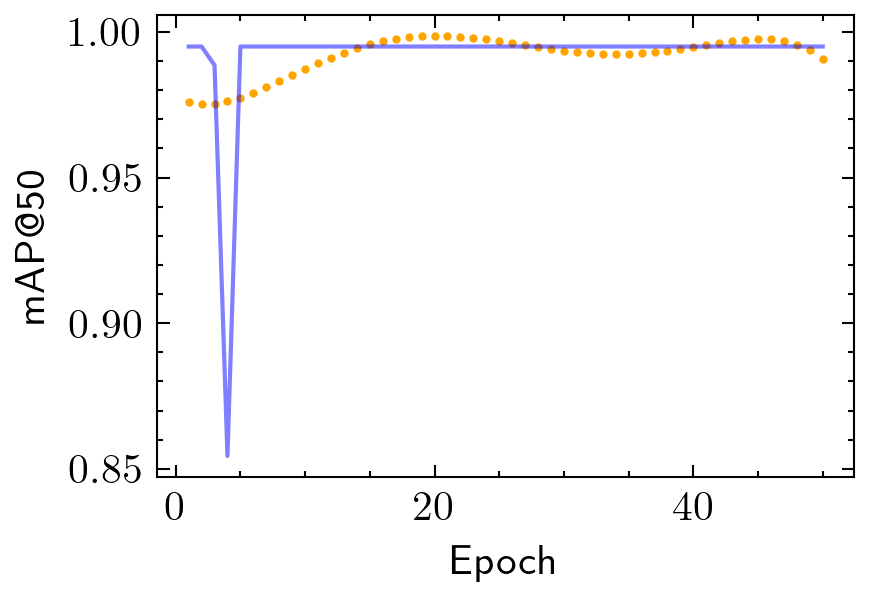
\includegraphics[width=\textwidth]{gambar/map50.png}
    (a)
  \end{minipage}
  \hfill
  % Second image
  \begin{minipage}[t]{0.48\textwidth}
    \centering
    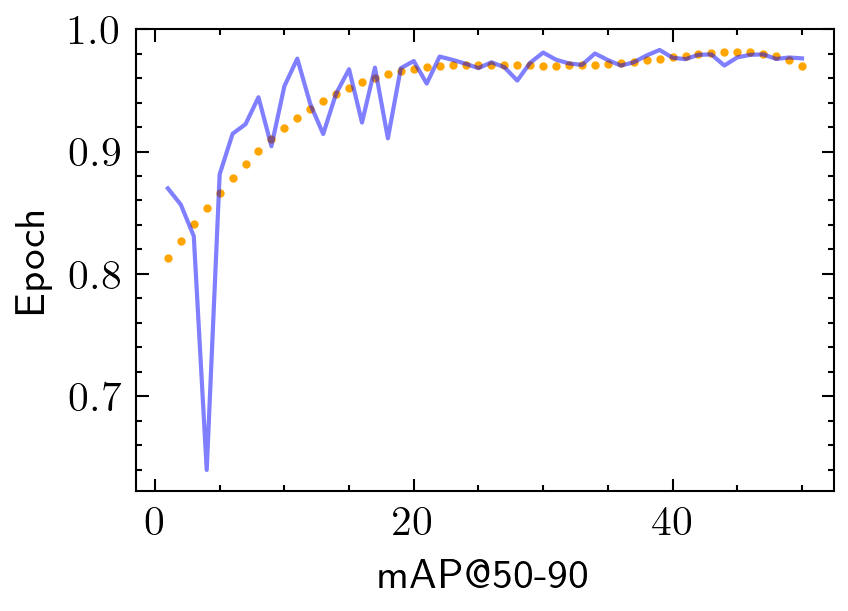
\includegraphics[width=\textwidth]{gambar/map5090.png}
    (b)
  \end{minipage}
  \caption{Grafik tren mAP: (a) mAP@50, (b) mAP@50-90}
  \label{fig:map}
  \vspace{-1em}
\end{figure}

Grafik tersebut menyajikan evaluasi performa model deteksi objek
menggunakan metrik mean Average Precision (mAP) seiring berjalannya
50 epoch pelatihan. Grafik di sebelah kiri, mAP@50, yang menggunakan
ambang batas IoU longgar (50\%), menunjukkan bahwa model dengan
sangat cepat mencapai performa puncak. Terlihat bahwa nilainya
melonjak mendekati 1.00 hanya dalam 10-15 epoch pertama lalu
cenderung datar, menandakan model mampu mempelajari cara mendeteksi
keberadaan objek secara umum dengan sangat cepat. Sebaliknya, grafik
di sebelah kanan, mAP@50-95, yang mengukur performa pada rentang
ambang batas IoU yang lebih ketat (50\% hingga 95\%), menunjukkan
kurva pembelajaran yang lebih bertahap dan konsisten. Peningkatan
yang lebih landai ini mengindikasikan bahwa model menggunakan
mayoritas waktu pelatihannya untuk terus-menerus menyempurnakan
presisi dan akurasi lokalisasi bounding box-nya. Secara keseluruhan,
pencapaian nilai mAP yang sangat tinggi pada kedua metrik di akhir
pelatihan menandakan model final yang dihasilkan tidak hanya mampu
mendeteksi objek, tetapi juga sangat akurat dalam menentukan
batas-batasnya. Hasil deteksi kontainer kimia pada data validasi
dapat dilihat pada Gambar \ref{fig:yolo-validasi}.

\begin{figure}[H]
  \centering
  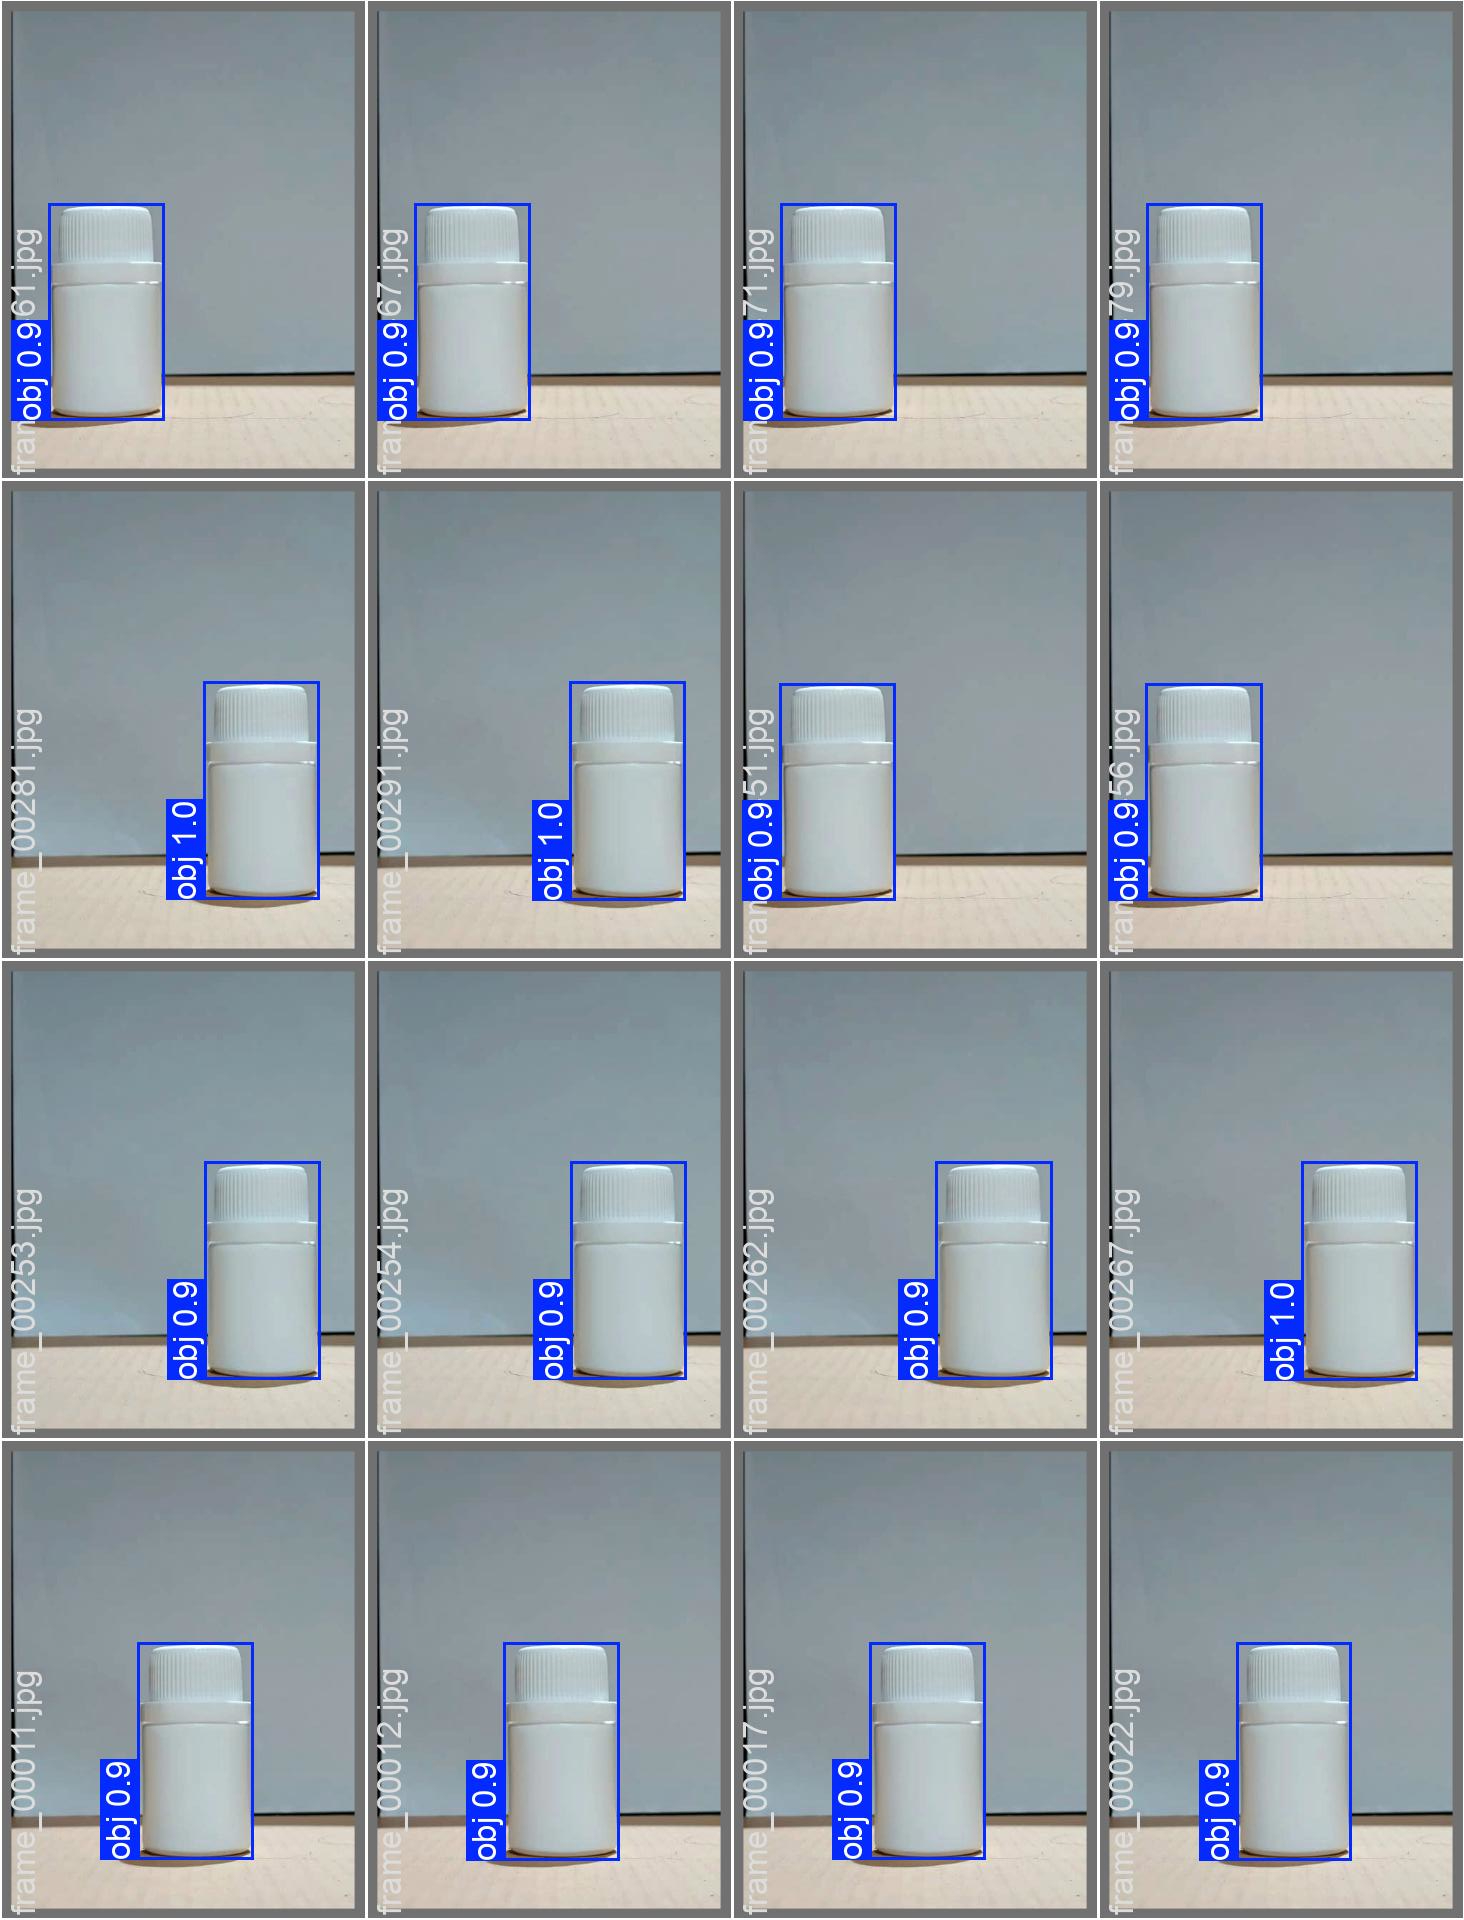
\includegraphics[width=0.7\textwidth]{gambar/yolo_validasi.jpg}
  \caption{Hasil prediksi YOLO pada data validasi}
  \label{fig:yolo-validasi}
\end{figure}
\vspace{-1em}

\vspace{1em}

\section{Hasil Perancangan Model Deteksi Kecacatan}
\subsection{Arsitektur Variational Autoencoder}
\subsection{Hasil Rekonstruksi dan Error}
\subsection{Penentuan Threshold Kecacatan}

\vspace{1em}

\section{Hasil Pengujian Sistem}

\chapter{KESIMPULAN}
\section{Kesimpulan}
Berdasarkan hasil perancangan, analisis, dan implementasi alat yang
telah digunakan, maka dapat diambil kesimpulan sebagai berikut:
\begin{enumerate}
  \item Model deteksi objek berbasis YOLO telah berhasil dirancang dan
    dilatih untuk mengenali kontainer kimia dengan akurasi dan
    presisi lokalisasi yang sangat tinggi. Kinerja model, yang
    dievaluasi menggunakan metrik \textit{mean Average Precision} (mAP),
    menunjukkan kemampuan yang sangat bagus dalam mendeteksi
    keberadaan objek dan menentukan \textit{bounding box} secara akurat.
  \item Model deteksi kecacatan menggunakan algoritma (CVAE) terbukti
    efektif dalam mengidentifikasi anomali visual pada permukaan
    kontainer. Model
    dilatih pada \textit{dataset} citra normal (tanpa cacat). Hasilnya, model
    mampu merekonstruksi citra normal dengan \textit{reconstruction
    error} yang rendah. Sebaliknya, kontainer cacat menghasilkan \textit{error}
    yang signifikan lebih tinggi. Penentuan ambang batas optimal sebesar
    0,007183 dilakukan melalui analisis kurva ROC. Ambang batas ini
    mampu mencapai tingkat akurasi 100\% pada 25 sampel uji.
  \item Sistem ini mampu menjalankan alur kerja otomasi secara
    menyeluruh: mulai dari akuisisi citra oleh kamera, identifikasi
    objek oleh YOLO, analisis kecacatan oleh CVAE, hingga penyortiran
    fisik kontainer oleh lengan robot ke area yang telah ditentukan
    (cacat atau normal). Dengan demikian, penelitian ini berhasil
    mendemonstrasikan kelayakan sebuah sistem inspeksi visual cerdas
    dan otomatis untuk penanganan kontainer di lingkungan industri terisolasi.
\end{enumerate}

\vspace{1em}

\section{Saran}
Alat yang telah dibuat memiliki potensi untuk dikembangkan lebih
lanjut. Berikut adalah beberapa saran untuk penelitian selanjutnya:
\begin{enumerate}
  \item Penelitian selanjutnya disarankan mencoba pendekatan
    \textit{supervised learning}, seperti \textit{convolutional
    neural network} (CNN)
    atau YOLO yang diadaptasi untuk klasifikasi cacat. Dengan adanya
    label pada data cacat, model diharapkan dapat mengenali berbagai
    jenis kerusakan secara lebih spesifik dan meningkatkan akurasi
    deteksi pada kondisi industri nyata.
  \item Kontrol pergerakan lengan robot pada prototipe ini masih
    bersifat \textit{hard-coded}, dengan sudut \textit{servo} yang ditentukan
    sebelumnya. Untuk meningkatkan fleksibilitas, disarankan
    menggunakan \textit{inverse kinematics}, sehingga lengan dapat secara
    dinamis menghitung sudut sendi untuk mencapai koordinat target
    (x, y, z). Dengan demikian, sistem mampu beradaptasi \textit{real-time}
    terhadap perubahan posisi objek tanpa perlu pemrograman ulang manual.
  \item Prototipe ini memanfaatkan satu kamera dengan sudut pandang
    tunggal untuk akuisisi citra. Keterbatasan ini menyebabkan
    inspeksi hanya dapat dilakukan pada permukaan yang terlihat oleh
    kamera, sehingga potensi adanya cacat di sisi lain kontainer akan
    terlewatkan. Untuk mengatasi hal ini, penelitian selanjutnya
    dapat berfokus pada pengembangan sistem inspeksi 360 derajat.
\end{enumerate}


\addcontentsline{toc}{chapter}{DAFTAR PUSTAKA}

\begin{thebibliography}{9}

  \bibitem[Jhang et al.(2024)]{1}
  Jhang, J. Y. \& Lin, C. J. 2024. Jhang, Jyun-Yu, \& Cheng-Jian
  Lin. Optimizing parameters of YOLO model through uniform
  experimental design for gripping tasks performed by an internet of
  things–based robotic arm. Internet of Things 27, 1-12. doi:
  10.1016/j.iot.2024.101332.

  \bibitem[Oaki et al.(2023)]{2}
  Oaki, J., Sugiyama, N., Ishihara, Y., Ooga, J., Kano, H. \& Ohno,
  H., 2023. Micro-Defect Inspection on Curved Surface Using a 6-DOF
  Robot Arm with One-Shot BRDF Imaging. IFAC-PapersOnLine 56(2),
  9354-9359. doi: 10.1016/j.ifacol.2023.10.224.

  \bibitem[Lin et al.(2024)]{3}
  Lin, C. J., Jhang, J. Y., Gao, Y. J. \& Huang, H. M., 2024.
  Vision-based Robotic Arm in Defect Detection and Object
  Classification Applications. Sensors \& Materials 36(2), 655-670.
  doi: 10.18494/SAM4683.

  \bibitem[Truong et al.(2024)]{4}
  Truong, A. M. \& Luong, H. Q., 2024. A non-destructive,
  autoencoder-based approach to detecting defects and contamination
  in reusable food packaging. Current Research in Food Science 8, 1-12.
  doi: 10.1016/j.crfs.2024.100758.

  \bibitem[Graetz et al.(2018)]{5}
  Graetz, G. \& Michaels, G., 2018. Robots at work. Review of
  economics and statistics 100(5), 753-768. doi: 10.1162/rest\_a\_00754.

  \bibitem[Gihleb et al.(2022)]{6}
  Gihleb, R., Giuntella, O., Stella, L. \& Wang, T., 2022.
  Industrial robots, workers’ safety, and health. Labour economics
  78, 1-12. doi: 10.1016/j.labeco.2022.102205.

  \bibitem[Tsai et al.(2021)]{7}
  Tsai, D. M. \& Jen, P. H. 2021., Autoencoder-based anomaly detection
  for surface defect inspection. Advanced Engineering Informatics 48,
  1-12. doi: 10.1016/j.aei.2021.101272.

  \bibitem[Chen et al.(2021)]{8}
  Chen, Y., Ding, Y., Zhao, F., Zhang, E., Wu, Z. \& Shao, L., 2021.
  Surface defect detection methods for industrial products: A review.
  Applied Sciences 11(16), 1-25. doi: 10.3390/app11167657.

  \bibitem[Liu et al.(2025)]{9}
  Liu, Y., Qiu, W., Fu, K., Chen, X., Wu, L. \& Sun, M., 2025. An
  improved YOLOv8 model and mask convolutional autoencoder for
  multi-scale defect detection of ceramic tiles. Measurement 248,
  1-11. doi: 10.1016/j.measurement.2025.116847.

  \bibitem[Wang et al.(2024)]{10}
  Wang, L., 2024. Robot arm grasping based on YOLOv5 in the
  perspective of automated production. Engineering Research Express,
  6(4), 1-12. doi:10.1088/2631-8695/ad88dc.

  \bibitem[Kato et al.(2022)]{11}
  Kato, H., Nagata, F., Murakami, Y. \& Koya, K., 2022. Partial depth
  estimation with single image using YOLO and CNN for robot arm
  control. IEEE International Conference on Mechatronics and
  Automation (ICMA), 1727-1731. IEEE. doi: 10.1109/ICMA54519.2022.9856055.

  \bibitem[Kim et al.(2021)]{12}
  Kim, M. \& Kim, S. 2021., YOLO-based robotic grasping. International
  Conference on Control, Automation and
  Systems (ICCAS) 21, 1120-1122. doi: 10.23919/ICCAS52745.2021.9649837.

  \bibitem[Jin et al.(2025)]{13}
  Jin, T., Han, X., Wang, P., Zhang, Z., Guo, J. \& Ding, F., 2025.
  Enhanced deep learning model for apple detection, localization, and
  counting in complex orchards for robotic arm-based harvesting.
  Smart Agricultural Technology 10, 1-25. doi: 10.1016/j.atech.2025.100784.

  \bibitem[Bionda et al.(2022)]{14}
  Bionda, A., Frittoli, L. \& Boracchi, G., 2022. Deep
  autoencoders for anomaly detection in textured images using
  CW-SSIM. International Conference on Image Analysis and
  Processing, 669-680. doi: 10.1007/978-3-031-06430-2\_56.

  \bibitem[Yun et al.(2023)]{15}
  Yun, H., Kim, H., Jeong, Y. H. \& Jun, M. B., 2023.
  Autoencoder-based anomaly detection of industrial robot arm using
  stethoscope based internal sound sensor. Journal of Intelligent
  Manufacturing 34(3), 1427-1444. doi: 10.1016/j.ymssp.2004.10.013.

  \bibitem[Jia et al.(2023)]{16}
  Jia, H. \& Liu, W., 2023. Anomaly detection in images with shared
  autoencoders. Frontiers in Neurorobotics 16, 1-11. doi:
  10.3389/fnbot.2022.1046867.

  \bibitem[Kozamernik et al.(2025)]{17}
  Kozamernik, N. \& Bračun, D., 2025. A novel FuseDecode Autoencoder
  for industrial visual inspection: Incremental anomaly detection
  improvement with gradual transition from unsupervised to
  mixed-supervision learning with reduced human effort. Computers in
  Industry 164, 1-19. doi: 10.1016/j.compind.2024.104198.

  \bibitem[Ruediger-Flore et al.(2024)]{18}
  Ruediger-Flore, P., Klar, M., Hussong, M., Mukherjee, A., Glatt,
  M. \& Aurich, J. C., 2024. Comparing Binary Classification and
  Autoencoders for Vision-Based Anomaly Detection in Material Flow.
  Procedia CIRP 121, 138-143. doi: 10.1016/j.procir.2023.09.241.

  \bibitem[Ragab et al.(2024)]{19}
  Ragab, M. G., Abdulkadir, S. J., Muneer, A., Alqushaibi, A.,
  Sumiea, E. H., Qureshi, R. et al., 2024. A
  comprehensive systematic review of YOLO for medical object
  detection (2018 to 2023). IEEE Access 12, 57815-57836. doi:
  10.1109/ACCESS.2024.3386826.

  \bibitem[Hussain(2024)]{20}
  Hussain, M., 2024. Unveiling each variant–a comprehensive review of
  yolo. IEEE access 12, 42816-42833. doi: 10.1109/ACCESS.2024.3378568.

  \bibitem[Padilla et al.(2021)]{21}
  Padilla, R., Passos, W. L., Dias, T. L., Netto, S. L., \& Da Silva,
  E. A., 2021. A comparative analysis of object detection metrics
  with a companion open-source toolkit. Electronics 10(3), 1-28. doi:
  10.3390/electronics10030279.

  \bibitem[Kaur dan Singh(2023)]{22}
  Kaur, R., \& Singh, S., 2023. A comprehensive review of object
  detection with deep learning. Digital Signal Processing 132, 1-17.
  doi: 10.1016/j.dsp.2022.103812.

  \bibitem[Casas et al.(2023)]{23}
  Casas, E., Ramos, L., Bendek, E., \& Rivas-Echeverría, F., 2023.
  Assessing the effectiveness of YOLO architectures for smoke and
  wildfire detection. IEEE Access 11, 96554-96583. doi:
  10.1109/ACCESS.2023.3312217.

  \bibitem[Cao et al.(2024)]{24}
  Cao, L., Shen, Z., \& Xu, S., 2024. Efficient forest fire detection
  based on an improved YOLO model. Visual Intelligence 2(20), 1-7.
  doi: 10.1007/s44267-024-00053-y.

  \bibitem[Mansour et al.(2021)]{25}
  Mansour, R. F., Escorcia-Gutierrez, J., Gamarra, M., Gupta, D.,
  Castillo, O., \& Kumar, S. 2021. Unsupervised deep learning based
  variational autoencoder model for COVID-19 diagnosis and
  classification. Pattern Recognition Letters, 151, 267-274.

  \bibitem[Kingma dan Welling(2013)]{25}
  Kingma, D. P., \& Welling, M. 2013. Auto-encoding
  variational bayes.

  \bibitem[Al Najjar(2024)]{27}
  Al Najjar, Y. 2024. Comparative analysis of image quality
  assessment metrics: MSE, PSNR, SSIM and FSIM. International Journal
  of Science and Research (IJSR), 13(3), 110-114.

  \bibitem[Nahm(2022)]{28}
  Nahm, F. S., 2022. Receiver operating characteristic curve:
  overview and practical use for clinicians. Korean journal of
  anesthesiology, 75(1), 25-36.

\end{thebibliography}

\end{document}
